Commençons par un type de droites que nous avons rencontré lors de la construction vue dans la section précédente. 

\begin{definition}
	Pour tous points $M$  et $N$ sur la parabole $\setgeo{P}: y = x^2$, la corde généralisée passant par $M$ et $N$ est la droite $\setgeo*{C}{MN}$ définie comme suit.
	\begin{enumerate}
		\item $\setgeo*{C}{MN} \eq[def] (MN)$ si $M \neq N$ .

		\item Sinon $\setgeo*{C}{MN}$ est la tangente en $M = N$ à la parabole $\setgeo{P}$ .
	\end{enumerate}
\end{definition}


\medskip

Comme pour le cercle, donnons-nous quatre points $A_1$ , $A_2$ , $A_3$ et $A_4$ sur la parabole $\setgeo{P}$ puis pour $n \in \NN_{\geq 5}$ définissons le point $A_n$ comme étant le point d'intersection, éventuellement double
\footnote{
	Une tangente à la parabole admet un point d'intersection double.
},
de la parabole $\setgeo{P}$ avec la parallèle à $\setgeo*{C}{A_{n-3} A_{n-4}}$ passant par $A_{n-1}$ .
Voici un exemple de tracé où il semblerait de nouveau que $A_7 = A_1$ . En testant d'autres situations
\footnote{
	Le lieu de téléchargement de ce document contient un fichier GeoGebra \texttt{base-tool-parabola.ggb} manipulable dynamiquement pour tester la conjecture.
},
cette conjecture se solidifie rapidement. Frappant ! Non ?
 

\vspace{1em}

\begin{center}
	\fbox{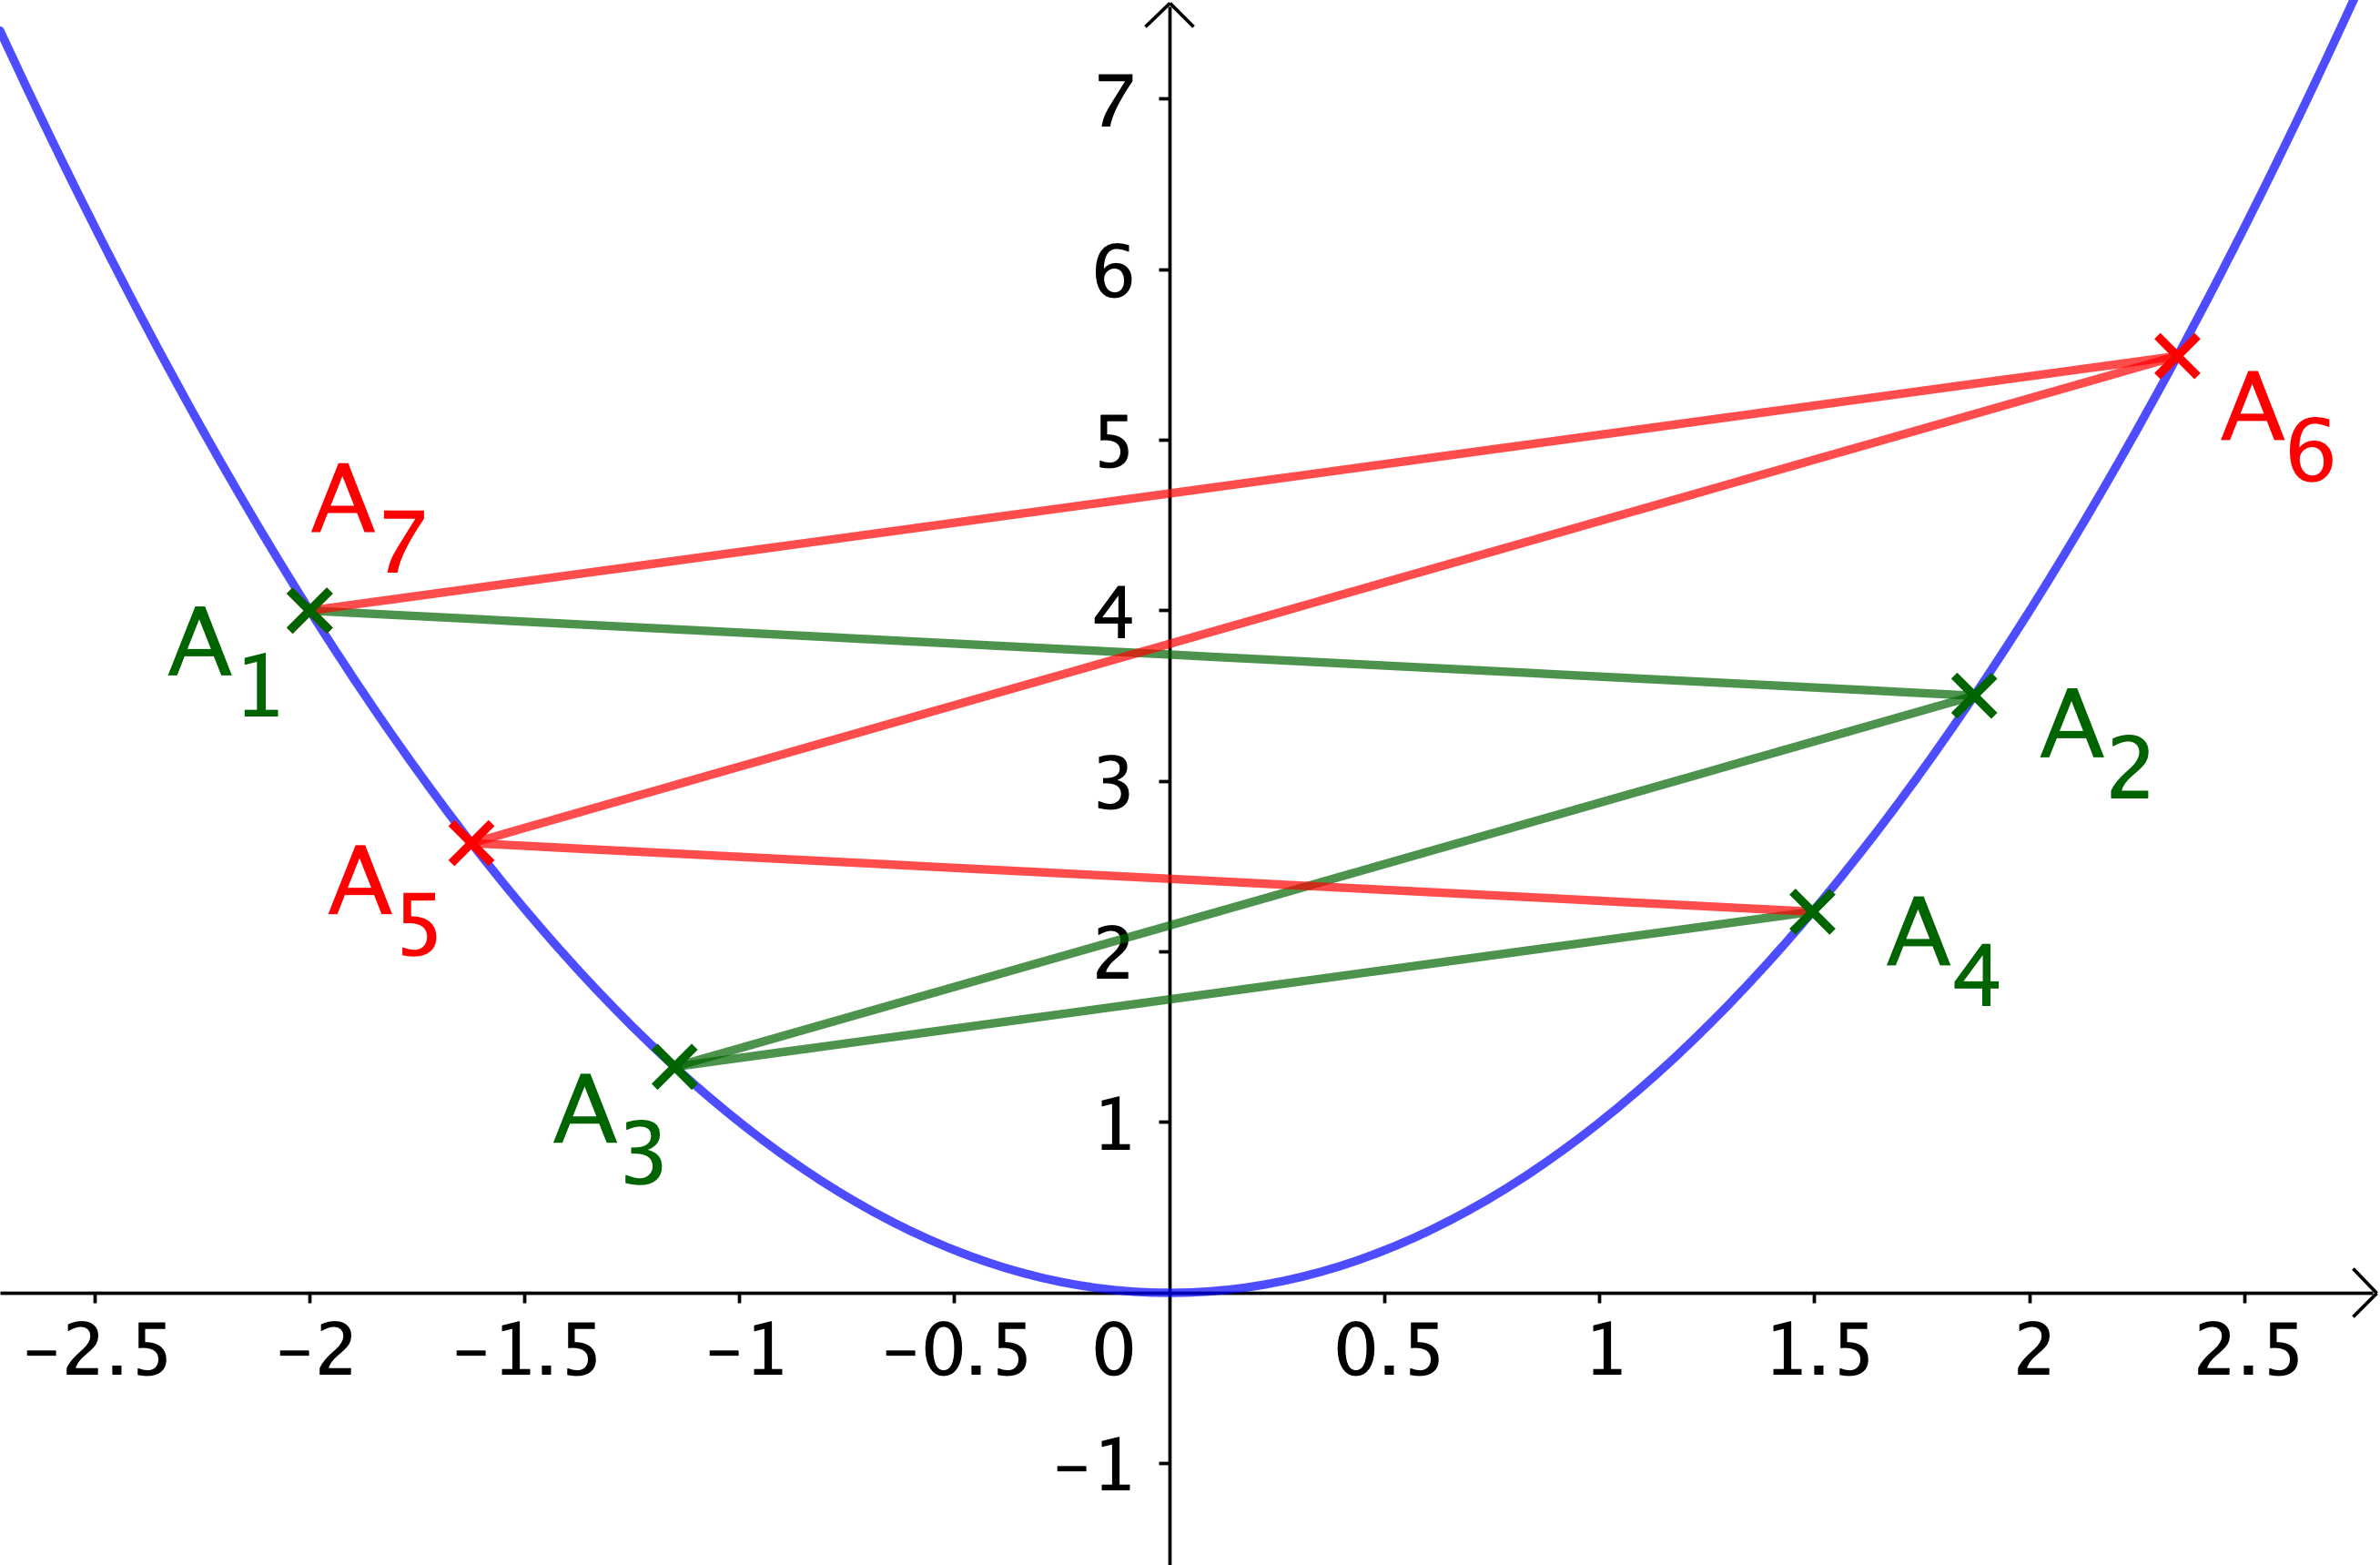
\includegraphics[scale = .8]{parabola/conjecture.png}}
\end{center}

\vspace{1em}

 
% ----------- %


La preuve va être ici des plus faciles grâce à quelques résultats simples d'analyse
\footnote{
	Le lecteur habitué notera que les raisonnements faits utilisent juste du calcul différentiel sur des polynômes à une variable. Nous avons donc une démonstration plus algébrique qu'analytique.
}.
En effet, la pente d'une corde généralisée $\setgeo*{C}{MN}$ est $x_M + y_N$ pour les raisons suivantes.
\begin{enumerate}
	\item Si $M \neq N$ , $\setgeo*{C}{MN} \eq[def] (MN)$ a pour pente $\frac{y_M - y_N}{x_M - x_N} = \frac{x_M^2 - x_N^2}{x_M - x_N} = x_M + y_N$ .

	\item Si $M = N$ , $\setgeo*{C}{MN}$ est la tangente en $M$ à la parabole $\setgeo{P}$ . Cette tangente a pour pente $2 x_M = x_M + y_N$ .
\end{enumerate}


\medskip

Comme avec le cercle, $\forall n \in \NN_{\geq 5}$ , 
$\setgeo*{C}{A_{n} A_{n-1}} \,/\!/\, \setgeo*{C}{A_{n-3} A_{n-4}}$ , et l'on en déduit ici les égalités suivantes où $x_i \eq[def] x_{(A_i)}$ .
\begin{itemize}[label=\small\textbullet]
	\item \textbf{[L1]} : 
	      $x_1 + x_{2} = x_{4} + x_{5}$

	\item \textbf{[L2]} : 
	      $x_2 + x_{3} = x_{5} + x_{6}$

	\item \textbf{[L3]} : 
	      $x_3 + x_{4} = x_{6} + x_{7}$
\end{itemize}


\medskip

Comme dans la section \ref{circle-proof-1}, ceci implique $x_1 = x_7$ , soit de façon équivalente $A_7 = A_1$ . Retomber sur le même système n'est pas que pur hasard. Rendez-vous à la section \ref{group} qui va lever le voile de cette mystérieuse coïncidence.
